\documentclass[a4paper,12pt]{article} % тип документа

\usepackage{tikz}
\usepackage[T2A]{fontenc}			% кодировка
\usepackage[utf8]{inputenc}			% кодировка исходного текста
\usepackage[english,russian]{babel}	% локализация и переносы
\usepackage{amsfonts,longtable}

% Математика
\usepackage{amsmath,amsfonts,amssymb,amsthm,mathtools} 


\usepackage{wasysym}

\title{Лабораторная работа 1.4.5 по курсу \\ "Общая физика"  \\ 
\vspace{0.2cm}
\vspace{4.5cm}
 \LARGE{\textbf{Изучение колебаний струны}}\vspace{5.5cm}}
\date{02.11.2018}
\usepackage{tikz}
\author{\vspace{0.2cm}Баринов Леонид}

\begin{document}
\maketitle
\newpage
\section{Аннотация} В работе прдеставлены измерения собвственных частот колебаний струны, провдено сравнение эксперментальных измерений с теоритической оценкой. Построены графики частоты $\nu$ гармоники для различных наятяжений $T$. Определена скорость волн $u$ бегущих по струне. Построен график зависимости квадрата скорости $u^2$ от силы натяжения $T$. Проведено сравнение $\rho_l$, полученное в эксперименте, со значением, указанным на установке. Также проведен анализ колебаний струны при частоте в два раза меньше частоты основной гармоники.

\section{Теоритические данные}
Струной в акустике называют однородную тонкую гибкую упругую нить. Примерами могут служить сильно натянутый шнур или трос, струны гитары, скрипки и других музыкальных инструментов. В данной работе изучаются попереченые колебания стальной гитарной струны, натянутой горизонтально и закрепленной между двумя неподвижными зажимами.

Основное свойство струны -- \textit{гибкость} -- обсуловлено тем, что ее поперечные размеры малы по сравнению с длиной. Это означает, что напряжение в струне может быть направлено только вдоль нее, и позволяет не учитывать изгибные напряжения, которые могли бы возникать при поперечных деформациях (то есть, при изгибе струны).

В натянутой струне возникает \textit{поперечная упругость}, т. е. способность сопротивляться всякому изменеию формы, происходящему без изменения объема. При вертикальном смещении приовзольного элемента струны, возникают силы, действующие на соседние элементы, и в результате вся струна приходит в движение в вертикальной плоскости, т. е. возбуждение бежит по струне. Передача возбуждения представляет собой \text{попереченые бегущие волны}, распространяющиеся с некоторой скоростью в обе стороны от места возбуждения. В ненатянутом сотоянии струна не обладает свойством попереченой упругсоти и поперечные волны на ней невозможны.

Рассмотрим гибкую однородную струну, в которой создано натяжение $T$, и получим диффернциальное уравнение, описывающее ее малые поперечные свободные колебания. Отметим, что если струна расположена горизонтально в поле тяжести, величина $T$ должна быть достаточна для того, чтобы в стостоянии равовесия струна не провисала, т. е. сила натяжения должна существенно превышать вес струны.

Направим ось $x$ вдоль струны в положении равновесия. Форму струны будем описывать функцией $y(x, t)$, определяющей ее вертикальное смещение в точке $x$ в момент времени $t$ (см Рис. 1). Угол наклона касательной к струне в точке $x$ относительно горизонтального направлениф обозначим как $\alpha$. В любой момент этот угол совпадает с углом наклона касательной к графику функции $y(x)$, то есть $tg\alpha = \frac{\delta y}{\delta x}$
\begin{figure}[h]
\centering
\includegraphics[scale=0.5]{5}
\caption{К выводу уравнения колебаний струны}
\end{figure}
Рассмотрим элементарный участок струны, находящийся в точке $x$, имеющий длину $\delta x$ и массу $\delta m = \rho_l\delta x$, где $\rho_l$ -- погонная плотность струны (масса на единицу длины). При отклонении от равовесия на выделенный элемент действуют силы наятжения $T_1$ и $T_2$, направленные по касательной к струне. Их вертикальная составляющая будет стремиться вернуть рассматриваемый участок струны к положению равновесия, придавая элементу некотрое вертикальное ускорение $\frac{\partial^2y}{\partial t^2}$. Заметим, что угол $\alpha$ зависит от координаты $x$ вдоль струны и различен в точках приложения сил $T_1$ и $T_2$. Таким образом, второй закон Ньютона для вертикального движения элемента струны:
\begin{equation}
\delta m \frac{\partial^2 y}{\partial t^2} = -T_1\sin\alpha_1 + T_2\sin\alpha_2
\end{equation}
Основываясь на предположении, что отклонения струны от положения равовесия малы, можем сделать ряд упрощений:
\begin{itemize}
\item Длина учатска струны в изогнутом состоянии практически равна длине участка в положении равновесия, поэтому добавочным напряжением вследствие удлинения струны можно пренебречь. Следовательно, силы $T_1$ и $T_2$ по модулю равны силе натяжения струны $T_1 \approx T_2 \approx T$
\item Углы наклона $\alpha$ малы, поэтому $\tg\alpha\approx\sin\alpha\approx\alpha$ и, следовательно, можно положить $\alpha \approx\frac{\partial y}{\partial x}$.
\end{itemize}
Разделим обе части уравнения движения (1) на $\sigma x$ и устремим размер элемента к нулю, $\delta x \rightarrow 0$. Тогда правая часть (1) примет вид 
\[\rho_l\frac{\partial^2 y}{\partial t^2} = \frac{T_2\sin\alpha_2-T_1\sin\alpha_1}{\delta x}\approx T\frac{\alpha_2 - \alpha_1}{\delta x} \rightarrow T\frac{\partial\alpha}{\partial x}\]
(в последнем переходе использовано определение проихводной функции как предела отношения приращения функции к приращению аргумента). Наконец, подставляя $\alpha = \frac{\partial y}{\partial x}$, и вводя обозначение:

\begin{equation}
u = \sqrt{\frac{T}{\rho_l}}
\end{equation}
что, как видно дальше, есть скорость распространения волн на струне, находим окончательно уравнение свободных малых поперечных колебаний струны:

\begin{equation}
\frac{\partial^2 y}{\partial t^2} = u^2\frac{\partial^2 y}{\partial x^2}
\end{equation}
Уравнение (3) называют волновым уравнением. Кроме волн на струне, оно может описывать волновые процессы в самых разных системах, в том числе волны в сплошных средах(звук), электромагнитные волны и т. д.
\subsection{Бегущие волны}
Решение дифференциального уравнения в частных производных (3) предмтавимо в виде суммы двух волн произвольной формы, бегущих в противоположные стороны со скоростями $\pm u$:
\begin{equation}
y(x, t) = y_1(x-ut)+y_2(x+ut),
\end{equation}
где $u$ -- скорость распространения волны (2), $y_1$ и $y_2$ -- проивзольные функции, вид которых в конкретной задаче определяется из начальных и граничных условий.

Особый интерес представляет случай гармонических волн:
\begin{equation}
y(x, t) = a\cos[k(x-ut)] + b\cos[k(x+ut)] = a\cos(\omega t-kx)+b\cos(wt+kx)
\end{equation}

Выражение (5) представляет собой супрепозицию двух гармонических волн, бегущих навстречу друг другу со скоростью
\begin{equation}
u = \frac{\omega}{k}=\nu\lambda
\end{equation}
Их \textit{длина волны} $\lambda = \frac{2\pi}{k}$, \textit{частота} $\nu = \frac{\omega}{2\pi}$. Величина $k = \frac{2\pi}{\lambda}$ называется волновым числом или пространственной частотой волны.
Заметим, что формула (2) означает, что скорость $u$ распространения поперечных волн на струне зависит только от силы натяжения струны $T$ и ее погонной плотности $\rho_l$.
\subsection{Собственные колебания струны. Стоячие волны}
Функция, описывающая стоячие волны:
\begin{equation}
y(x, t) = 2a \sin kx\cdot \sin\omega t
\end{equation}
Видно, что стоячая волна может быть получена как сумма (интерференция) двух гармонических бегущих волн, имеющих равную амплитуду и двужущихся навстречу друг другу.

Как видоно из (7), точки струны, в которых $sinkx = 0$, в любой момент времени неподвижны. Такие точки называются узлами. Остальные точки совершают в вертикальной плоскости гармонические колебания с частотой
\[\nu = \frac{\omega}{2\pi}=\frac{u}{\lambda}\]
Амплитуда колебаний распределена вдоль струны по гармоническому закону: $y_0(x) = 2a\sin kx$. В точках, нде $\sin kx = 1$, амплитуда колебаний максимальна -- они называются пучностями. Между двумя соседними узлами все участки струны колеблются в фазу (их скорости имеют одинаковое направление), а при переходе через узел фаза колебаний меняется на $\pi$ вследствие изменения знакак $\sin kx$.

Исользуя второе граничное условие $y(L, t)=0$ (точки крепления струны должны быть узлами стоячей волны), найдем условие образования стоячих волн на струне: $y(x, t) = 2a\sin kL\cdot \sin \omega t = 0$, откуда
\[\sin kL = 0 \rightarrow kL = n\frac{\pi}{2},  n\in \mathbb{N}\] 
Таким образом, стоячие волны на струне с закрепленными концами могут образовываться только если на длине струны укладыается целое число полуволн:
\begin{equation}
L = \frac{\lambda_n}{2}n
\end{equation}
Поскольку длина волны однозначно связана с ее частотой, струна может колебаться только с определенными частотами:
\begin{equation}
\nu_n = \frac{u}{\lambda_n}=\frac{n}{2L}\sqrt{\frac{T}{\rho_l}}, n\in \mathbb{N}
\end{equation}
Набор (спектр) расзерешенных частот $\nu_n$ называют собственными частотами колебаний струны. Режим колебаний соответсвующий каждой из частот $\nu_n$, называется собственной (или нормальной) модой колебаний. Проивзольное колебание струны может быть представленно в виде суперпозиции ее собственных колебаний. Наименьшая частота $\nu_1$ называется также основным тоном (или первой гармоникой), а остальные ($\nu_2 = 2\nu_1, \nu_3 = 3\nu_1, ...)$ - обертонами (высшими грамониками). Термин "гармоника иногда употребляется в общем смысле -- как элементарная составляющая сложного гармонического колебания.

На Рис. 2 показана картина стоячих волн для $n = 1, 2, 3$. Заметим, что число $n$ определяет число пучностей (но не узлов!) колеблющейся струны.

Таким образом спектр собственных частот струны определен ее погонной плотностью $\rho_l$, силой натяжения $T$ и длиной струны $L$ (отдельно отметим, что собственные частоты не зависят от модуля Юнга материала струны).
\begin{figure}[h]
\centering
\includegraphics[scale=0.5]{2}
\caption{Стоячие волны (собственные моды колебаний струны) для $n =1, 2, 3$}
\end{figure}
\subsection{Возбуждение колебаний струны}
При колебаниях реальной струны всегда имеет место потеря энергии (часть теряется вследствие трения о воздух, другая часть уходит через неиделаьно закрепленные концы струны и т. д.). Поддержание незатухающих колебаний в струне может осуществляться точенчным источником, в качестве которого в данной работе использует электромагнитный вибратор. При этом возникает необходимость переноса энергии от источника по всей струне.

Рассмотрим вопрос о передаче энергии по струне. В стоячей волне поток энергии вдоль струны отсутствует -- колебательная энергия, заключенная в отрезке струны между двумя соседними узлами, не транспортируется в другие части струны. В каждом таком отрезке проиходит перодическое (дважды за период) превращение кинетической энергии в потенциальную и обратно. Передача энергии между различными участками струны возможно только благодаря бегущим волнам, которые, однако, в рассмотренной выше идеальной модели струны не возникают. Парадокс снимается, если учесть, что из-за потерь энергии при отражении волны от концов не проиходит полной компенсации пдающей и отраженной волны, поэтому к стоячей волне на струне добавляется малая бегущая компонента -- именно она служит "разносчиком" энргии по всей системе. 

Для эффективной раскачки колебаний используется явление резонанса -- вынуждающая частота $\nu$ должна совпадать с одной из собственных частот струны $\nu_n$ (см. (9)). Когда потери энергии в точности компенсируются энергией, поступающей от вибратора, колебания струны становятся стационарными и на ней можно наблюдать стоячие волны. Если потери энергии за период малы по сравнению с запасом колебательной энергии в струне, то искажение стоячих волн бегущей волной не существенно — наложение бегущей волны малой амплитуды на стоячую визуально приводит к незначительному «размытию» узлов. Для достижения максимального эффекта от вибратора, его следует располагать вблизи узловой точки. Это можно показать из следующих элементарных соображений. Пусть вибратор, размещённый в точке $x_0$, способен раскачать соответствующий элемент струны до амплитуды . Если частота вибратора близка к резонансной (т.е. собственной), то как следует из (7), амплитуда колебаний струны в пучности будет равна $2a = \frac{A}{\sin kx_0}$. Таким образом, максимальная раскачка струны достигается, если значение $\sin kx_0$ устремить к нулю, что и соответсвует положениям узлов (из идеализированной модели струны следует, что при размещении вибратора в узле амплитуда колебаний устремится к бесконечности, однако в реальности она ограничивается силами трения и нелинейными эффектами).

Заметим также, что при наблюдении стоячих волн важно, чтобы колебания происходили в одной (вертикальной) плоскости, т. е. были поляризованы. Кроме того, важно, чтобы колебания струны проиходили с малой амплитудой, поскольку при сильном возбуждении нарушаются условия применимости волнового уравнения (3), и в опыте наблюдаются искажения, связанные с нелинейными эффектами.
\section{Оборудование и инструментальная погрешность:} Закрепленная на станине стальная струна, набор грузов, электромагнитные датчики, звуковой генератор, двухканальный осциллограф, частомер.\\
Значения величин, указанных на установке:
Диаметр струны:\\
\[d = 0,3\text{мм}\]
Масса пастины:
\[m_\text{пл} = 5,1\text{г}\]
Масса  крюка:
\[m_\text{кр} = 2,588\text{г}\]
Масса платформы:
\[m_{\text{плат}}=111,6\text{г}\]
Масса подвеса $m_\text{п}=m_\text{пл}+m_\text{кр}+m_{\text{плат}}$
\[m_\text{п}=	119,3\text{г}\]
Погонная плотность:
\[\rho_l = 568,4\frac{\text{мг}}{\text{г}}\]

Длина струны:
\[L = 50\text{см}\]
Погрешность измерения длины:
\[\sigma_L = 1\text{мм}\]
Погрешность измерения частоты:
\[\sigma_\nu=2\text{Гц}\]
\section{Экспериментальная установка:}
Схема установки приведена на Рис. 3. Стальная гитарная струна 1 закрепляется в горизонатльной положении между двумя стойками с зажимами 2 и 3, расположенными на массивной станине 4. Один конец струны закреплен в зажиме 2 неподвижно. К противоположному концу струны, перекинутому через блок, прикреплена платформа с грузами 5, создающими натяжение струны. Зажим 3 можно передвигать по станине, устанавливая требуемую длину струны. Возбуждение и регистрация колебаний струны осуществяются с помощью электромагнитных датчиков (вибраторов), расположенных на станине под струной. Электромагнитный датчик 6 подключен к звуковому генератору 7 и служит для возбуждения колебаний струны, частота которых измеряется с помощью частотомера 10 (в некоторых установках частомер встроен в генератор). Колебания струны регитрируются с помощью электромагнитного датчика 8, сигнал которого передается на вход осциллографа 9. Разъемы, через которые датчики с помощью кабелей соединяются с генератором и осциллографом, расположены на корпусе станины.
\begin{figure}[h]
\centering
\includegraphics[scale=0.5]{1}
\caption{Экспериментальная установка}
\end{figure}
\subsection{Принцип работы датчиков}
Устройство и внешний вид электромагнитного датчика показаны на Рис. 4. В пластмассовом корпусе закреплен подковообразный магнит. На полюсах магнита намотаны соединенные последовательно катушки перменного тока, который подается с генератора, Магнитное поле в зазоре мжеду полюсами электромагнита складывается из поля постоянного магнита $B_0$ и малой добавочной сотавляющей поля катушей $B_\sim \ll B_0$. Сила, скоторой электромагнит действует на стальную (магнитную) струну, попорциональна квадрату индукции $B$ суммарного поля в зазоре электромагнита:
\[F \propto (B_0+B_\sim)^2 \approx B_0^2 + 2B_0B_\sim.\]
Отсюда видно, что при $B_\sim \ll B_0$ сила $F$ линейно зависит от переменного поля $B_\sim$ , а значит и от тока в катушках (т. к. $B_\sim \propto I_\sim)$, и поэтому частота переменной силы $F_\sim \propto 2B_0B_\sim \propto I_\sim$, действующей на струну, совпадает с частотой генератора. То есть участок струны, расположенный над электромагнитом, совершает колебательное движене в вертикальной плоскости с частотой задающего генератора. Колебания далее передаются по всей струне и, если частота колебаний совпадает с одной из собственных частот струны, на струне устанавливается стоячая волна. Колеблющаяся струна возбуждает в регитрирующей катушке переменную ЭДС с амплитудой, пропрциональной амлпитуде колебаний струны. Сигнал ЭДС измеряется с помощью осциллографа.
\begin{figure}[h]
\centering
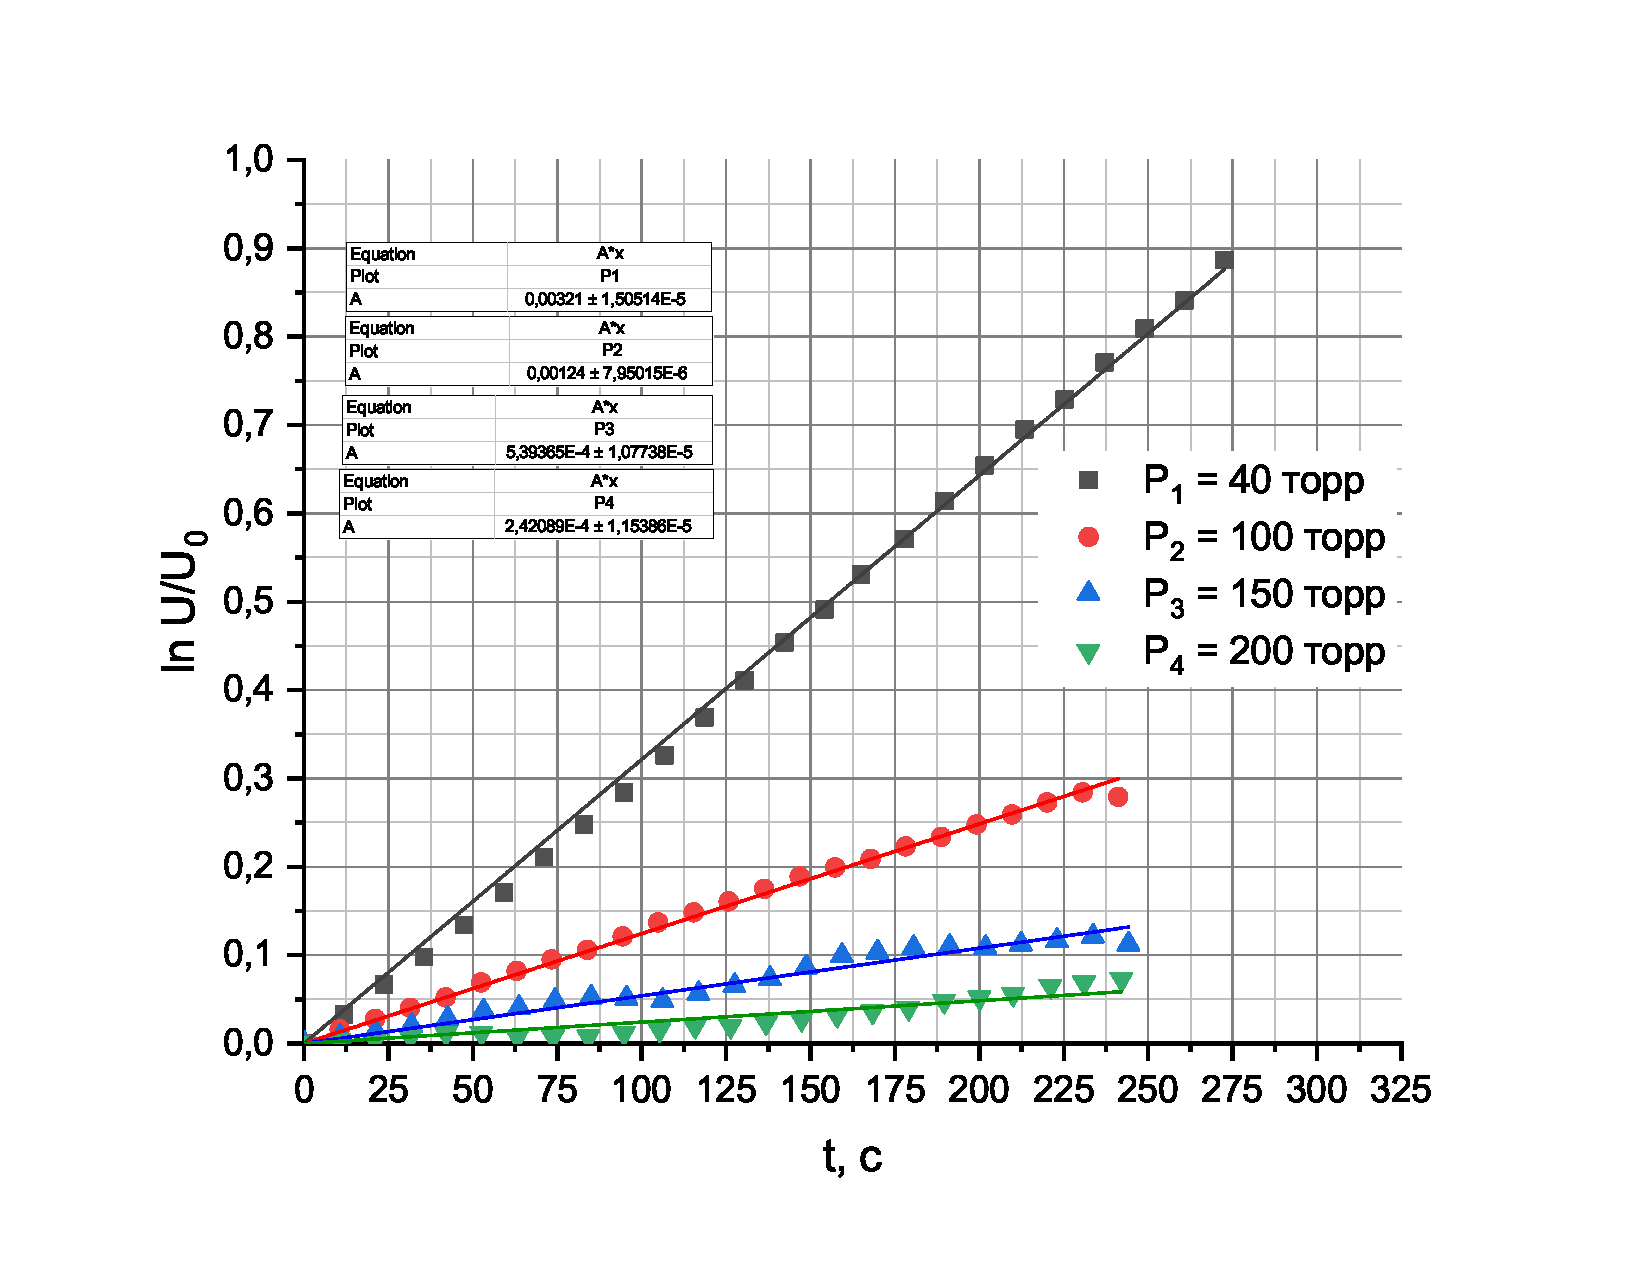
\includegraphics[scale=0.4]{6}
\caption{Электромагнитный датчик: а) вид спереди, б) вид сверху}
\end{figure}

Отметим, что магнитное поле наиболее однородно по координате в центральной части электромагнита, поэтому датчики должны быть повернуты так, чтобы струна располагалась в центральной части перпендикулярно к полюсам магнита. Возбуждающий датчик следует расположить вблизи неподвижного конца струны (ближе к узлу), а регитрирующий -- в пучности.
\subsection{Измерения с помощью осциллографа}
Дли регистрации колебаний струны в работе используется электронный осциллограф, соединенный с электромагнитным датчиком 8. Он позволяет регистрировать колебания в случаях, когда это невозможно сделать визуально. Также с помощью оциллографа можно измерять амплитуду возбуждения и форму сигнала, что дает возможность установить, является ли режим возбуждения стоячих волн линейным, иными словами, имеет ли место прямая пропорциональность между силой возбуждения и амплитудой колебаний струны, и не возникает ли отклонений от закона (7).

 Контролировать величину и форму сигнала колебаний струны на экране осциллографа можно несколькими способами: в одноканальном и двухканальном режимах работы осциллографа -- по временной равертке сигналов, а такжу в режиме сложения двух взаимно перпендикулярных сигналов -- основного и опорного


При возбуждении стоячей волны на экране осциллографа в режиме развертки должен появиться сигнал синусоидально формы. При чрезмерном возбуждении вид синусоиды искажается, что свидетельствует об отклонении от линейного режима. В двухканальном режиме осциллографа можно сравнить опорный (подаваемый одновременно на возбудитель колебаний 6 и канал CH1 осциллографа) и основной (снимаемый с датчика 8) сигналы — в отсутствие нелинейных искажений они должны совпадать. Кроме того, в режиме сложения сигналов (X–Y) на экране должен прорисовываться эллипс правильной формы.

Дополнительным критерием того, что частота гармоники определена верно, является симметричность «резонансной кривой» — амплитудно-частотной характеристики системы (Рис. 5). А именно, при подходе к резонансной частоте со стороны как высоких, так и со стороны низких частот, макси-мум сигнала наблюдается при одном и том же значении частоты.
\section{Результаты измерений и обработка данных}
Силы натяжения изменяются количеством дисков, находящихся на платформе. В Таблице 1 находится информация о суммарной массе дисков на платформе. В следующей строке посчитана сила натяжения струны по формуле $T_n = (m_n+m_\text{п})g$. В третьей строке произведены вычисления $u$ скорости распространения волны по формуле  (2). В следующей строке расчитана частота $\nu_\text{осн}$ основной гармоники по формуле (9). Погршеность $\sigma_L$ мала по сравнению с $L$, пренебрежем ее вкладом. 
\newpage
\begin{table}[h]
\centering
\begin{tabular}{|c|c|c|c|c|c|c|}
\hline
$\text{№}$ & 1 & 2 & 3 & 4 & 5 & 6 \\ \hline
$m,\text{г}$ & 920,7 & 1415,8 & 1750,1 & 2232,1 & 2729,3 & 3178,4 \\ \hline
$T, H$ &10,4 & 15,351 & 18,694 & 23,514 & 28,486 & 32,977\\ \hline
$\nu_\text{осн}, \text{Гц}$ & 135 & 164 & 181 & 203 & 224 & 240\\ \hline

\end{tabular}
\caption {Вычисление натяжения струны и частоты основной гармоники при данной силе натяжения струны}
\end{table}


С помощью осциллографа находим частоты гармоник. Начиная с первой,  заканчивая десятой. Результаты заносим в Таблицу 2. Номер $\nu$ сопоставляется с номером $T$.

\begin{table}[h]
\centering
\begin{tabular}{|c|c|c|c|c|c|c|c|c|c|c|}
\hline
$n$ & 1 & 2 & 3 & 4 & 5 & 6 & 7 & 8 & 9 & 10\\ \hline
$\nu_1, \text{Гц}$ & 139 & 279 & 418 & 559 & 699 & 841 & 983 & 1126 & 1270 & 1417\\ \hline
$\nu_2, \text{Гц}$ & 165 & 330 & 496 & 662 & 828 & 993 & 1162 & 1329 & 1485 & 1667\\ \hline
$\nu_3, \text{Гц}$ & 183 & 366 & 550 & 734 & 919 & 1103 & 1289 & 1472 & 1661 & 1846\\ \hline
$\nu_4, \text{Гц}$ & 201 & 402 & 604 & 804 & 1007 & 1208 & 1412 & 1614 & 1819 & 2023 \\ \hline
$\nu_5, \text{Гц}$ & 224 & 448 & 672 & 896 & 1121 & 1345 & 1572 & 1797 & 2025 & 2251\\ \hline
$\nu_6, \text{Гц}$ & 238 & 476 & 715 & 954 & 1193 & 1431 & 1672 & 1912 & 2153 & 2394\\ \hline
\end{tabular}
\caption{Измерение частоты для $n$ количества полуволн при натяженияx струны $T$}
\end{table}
По результатам $\nu$, представленным в Таблице 2, посчитаем скорость распространения волны по формуле (6), где $\lambda=2L/n$. Найдем среднее значение скорости и ее погрешность. Результаты занесем в  Таблицу 3. Систематическая погрешность пренебрижимо мала по сравнению со случайной.
\begin{table}[h]
\centering
\begin{tabular}{|c|c|c|c|c|c|c|}
\hline
$\text{№}$ & 1 & 2 & 3 & 4 & 5 & 6\\ \hline
$u, \text{м/с}$ & 140,15 & 165,58 & 183,78 & 201,49 & 224,37 & 238,64\\ \hline
$\sigma_u, \text{м/с}$ & 0,32 & 0,14 & 0,15 & 0,10 & 0,08 & 0,10\\ \hline
\end{tabular}
\caption{Скорость распространения волны и ее погрешность}
\end{table}

По данным Таблицы 2 построим графики зависимости частоты от номера гармоники для различных натяжений $T$. (Рис. 5). Также построим график зависимости квадрата скорости $u^2$ от силы натяжения $T$(Рис. 6) по данным Таблицы 1 и Таблицы 3. Погрешности в каждом из графиков укладываются в размеры точек 
\newpage
\begin{figure}[!h]
\centering
\includegraphics[scale=0.4]{11}
\caption{Графики зависимости частоты $\nu_n$ от номера $n$ гармоники для различных натяжений $T$}
\end{figure}
\begin{figure}[!h]
\centering
\includegraphics[scale=0.28]{12}
\caption{Зависимость силы натяжения $T$ от квдарата скорости $u^2$}
\end{figure}
Используя формулу (2) вычислим погонную плотность струны. Усредним результат и надйем погрешность.
\[\rho_l = 561\pm17\frac{\text{мг}}{\text{м}}\]

Благодаря высокой добротности струны, возможно возбуждение ее колебаний при кратных частотах генератора, меньших, чем частота основной гармоники. С помщью осциллографа найдем значение частоты $\nu_{\frac{1}{2}}$.  На экране осциллографа в режиме $X-Y$ наблюдается фигура Лиссажу с одним самопересечением. (Рис. 7)
\begin{figure}[h]
\centering
\includegraphics[scale=0.4]{10}
\caption{Фигура Лиссажу с одним самопересеченим при $\nu_{\frac{1}{2}} \approx \frac{\nu_1}{2}$}
\end{figure}

Частота $\nu_{\frac{1}{2}}=118,9 \text{Гц}$. Эта точка также отмечена на графике зависимости частоты от номера гаромоники. (Рис. 5)
\section{Обсуждение результатов и выводы}
Большая часть значений частот основной гармоники $\nu_\text{осн}$  в пределах погрешности совпадает с теоритической оценкой. (Сравнение значений $\nu_\text{осн}$ в Таблице 1 cо вторым столбцом в Таблице 2). 

Значения частот, соответсвующих номеру гармоники, при неизменном натяжении отражают прямо пропорциональную зависимость частоты от номера гармоники (Рис. 5), что подтверждает формулу (9).

График зависимости силы натяжения $T$ от квадрата скорости $u^2$(Рис. 6) свидетельствует о прямопропрциональной зависимости между этими величинами, что соответствует формуле (2).

В работе было получено значение погонной плотности $\rho_l$
\[\rho_l = 561\pm17\frac{\text{мг}}{\text{м}}\]
Экспериментальное значение в пределах погрешности совпадает со значением $\rho_l$, указанным на установке.

В случае, когда частота колебаний струны равна половине частоты основной гармоники, колебания струны соответствуют пересечению двух синусоид, исходящих из закрепленных концов, длины волн которых равны четырем длинам струны. Вследствие этого струна будет колебаться с частатой в два раза меньшей, чем частота генератора. Такому соотнешению частот соответсвует фигура Лиссажу с одним самопересечением (Рис. 7).
\end{document}